\chapter{Marco Teórico} \label{ch:m_teorico}

% estructura
\section{Sistemas de Conducción Autónoma}
Un sistema de conducción autónoma es una combinación de varios componentes o subsistemas donde las tareas 
de percepción, toma de decisiones y operación de un vehículo son desarrolladas por un sistema electrónico en lugar
de un conductor humano. Usualmente, un sistema de conducción autónoma incluye varios subsistemas de automatización 
que operan de manera conjunta y coordinada para poder tomar el control total o parcial del vehículo. 

En algunas ocasiones, la automía del control se implementa de manera condicional, es decir, que el sistema toma 
el control del vehículo para ciertas situaciones pero no todo el tiempo como por ejemplo sistemas de estabilización 
de frenos o prevención de impactos. Este tipo de sistemas se ha ido desarrollando e implementando en vehículos comerciales 
de manera paulatina pero todavía no existe un vehículo completamente autónomo circulando por las calles o carreteras. Notese
que los términos autonomía y automatización se usan de manera intercambiable en este contexto.

    \subsection{Niveles de Autonomía}
    Debido al creciente interés e inversión en el desarrolo de sistemas de conducción autónoma se ha establecido 
    una manera de categorizar los niveles de automatización de la conducción por parte de  la Sociedad de Ingenieros en Automoción
    (SAE, por sus siglas en inglés) en la que se definen seis niveles de automatización en vehículos terrestres, acuáticos y aéreos.

        \subsubsection{Nivel 0: Sin automatización}
        El conductor está en completo control de todas las funciones del vehículo en todo momento, no existe intervención 
        de ningún sistema automatizado en el control. Sistemas de alerta de colisión o pérdida de carril entran en esta categoría.
        \subsubsection{Nivel 1: Conducción asistida}
        El conductor tiene el control del vehículo, pero el sistema puede modificar la aceleración o dirección del mismo. Los 
        sistemas de control de velocidad de crucero caen en esta categoría.
        \subsubsection{Nivel 2: Automatización parcial}
        El conductor debe poder ser capaz de tomar el control del vehículo si ciertas se necesitan ciertas correcciones, pero  
        ya no está en control de la aceleración y dirección del vehículo directamente. Es importante resaltar que desde los
        niveles 0 al 2 el conductor no puede estar distraido en ningún momento de la conducción. Los sistemas de parqueo 
        automático representan un buen ejemplo de sistemas de Nivel 2.
        \subsubsection{Nivel 3: Automatización condicional}
        El sistema automatizado tiene el control del vehículo, tanto de la aceleración, dirección así como también del monitoreo 
        del entorno bajo condiciones específicas. El conductor debe estar preparado para intervenir cuando el sistema así lo 
        requiera, por tanto, se permiten distracciones ocasionales. Uno de los sistemas recientemente implementados que cae en esta 
        categoría es el sistema \textit{autopilot} de los vehículos de Tesla Motors. % agregar referencia
        \subsubsection{Nivel 4: Automatización elevada}
        El sistema está en completo control del vehículo y la presencia humana ya no es necesaria, sin embargo, la operación autónoma 
        del vehículo está limitada a condiciones específicas. Si las actuales condiciones del entorno sobrepasan las fronteras 
        de rendimiento definidas, el vehículo puede desplegar un protocolo o secuencia de emergencia. Actualmente el desarrollo 
        de vehículos autónomos o \textit{self driving cars} se enfoca en este nivel. 
        \subsubsection{Nivel 5: Automatización completa}
        El sistema está en completo control del vehículo y la presencia humana no es necesaria en absoluto. El sistema es capaz 
        de proveer las mismas características que en el Nivel 4, pero en esta ocasión puede operar al vehículo en todas las condiciones.
        En este nivel, el conductor pasa a ser un pasajero en el vehículo. Actualmente, no existen sistemas que operen en este nivel.

    La relación entre la responsabilidad del sistema y el conductor en los distintos niveles se puede apreciar en la 
    Tabla \ref{tbl:niveles}:
    
        \begin{table}[!h]
            \centering
            \resizebox{\textwidth}{!}{%
            \begin{tabular}{@{}|c|l|c|c|c|c|@{}}
            \toprule
            \textbf{Nivel SAE} & \textbf{Denominación}      & \textbf{\begin{tabular}[c]{@{}l@{}}Ejecución de aceleración \\ y dirección\end{tabular}} & \textbf{\begin{tabular}[c]{@{}l@{}}Monitoreo del \\ entorno\end{tabular}} & \textbf{\begin{tabular}[c]{@{}l@{}}Responsable en \\ condiciones difíciles\end{tabular}} & \textbf{\begin{tabular}[c]{@{}l@{}}Modos de \\ conducción\end{tabular}} \\ \midrule
            0                  & Sin Automatización         & Humano                                                                                   & \multirow{3}{*}{Humano}                                                   & \multirow{4}{*}{Humano}                                                                  & Ninguno                                                                 \\ \cmidrule(r){1-3} \cmidrule(l){6-6} 
            1                  & Conducción asistida        & Humano y sistema                                                                         &                                                                           &                                                                                          & \multirow{3}{*}{Algunos Modos}                                          \\ \cmidrule(r){1-3}
            2                  & Automatización parcial     & \multirow{4}{*}{Sistema}                                                                 &                                                                           &                                                                                          &                                                                         \\ \cmidrule(r){1-2} \cmidrule(lr){4-4}
            3                  & Automatización condicional &                                                                                          & \multirow{3}{*}{Sistema}                                                  &                                                                                          &                                                                         \\ \cmidrule(r){1-2} \cmidrule(l){5-6} 
            4                  & Automatización elevada     &                                                                                          &                                                                           & \multirow{2}{*}{Sistema}                                                                 & Varios Modos                                                            \\ \cmidrule(r){1-2} \cmidrule(l){6-6} 
            5                  & Automatización completa    &                                                                                          &                                                                           &                                                                                          & Todos los Modos                                                         \\ \bottomrule
            \end{tabular}%
            }
            \caption{Niveles de automatización según SAE. Fuente: SAE} % TODO: referencia
            \label{tbl:niveles}
            \end{table}

    \subsection{Arquitectura de un sistema de conducción autónoma}
    % \subsection{Aprendizaje Profundo}


\section{Visión por computador}
-
    \subsection{Procesamiento de imágenes}
    \subsection{Filtrado}

\section{Redes Neuronales Artificiales}

    \subsection{Aprendizaje Automático}
    El aprendizaje automático es un subcampo de la inteligencia artificial que intenta extraer 
    patrones mediante un proceso de \textit{aprendizaje} a partir de datos \cite{Mitchell1990}. Este proceso 
    de aprendizaje se define de acuerdo a una \textbf{tarea específica} $T$ que intenta aprenderse en base 
    a \textbf{experiencia pasada} $E$ tomando como referencia una \textbf{medida de rendimiento} $P$ . 
    Dentro de esta definición, se puede listar varios ejemplos de tareas de aprendizaje que usualmente se resuelven  
    usando los conceptos del aprendizaje automático o también llamado \textit{machine learning}:
    \\
    \\
    \begin{itemize}
        \item \textbf{Un algoritmo de aprendizaje que pueda jugar ajedrez:}
        \begin{itemize}
            \item \textbf{Tarea $T$:} Jugar Ajedrez.
            \item \textbf{Medida de Rendimiento $P$:} Porcentaje de partidas ganadas contra el oponente.
            \item \textbf{Experiencia $E$:} Información de varias partidas de práctica.
        \end{itemize}
        
        \item \textbf{Un algoritmo de aprendizaje que pueda reconocer dígitos manuscritos:}
        \begin{itemize}
            \item \textbf{Tarea $T$:} Reconocer y clasificar dígitos manuscritos dentro de una imagen.
            \item \textbf{Medida de Rendimiento $P$:} Porcentaje de dígitos correctamente clasificados.
            \item \textbf{Experiencia $E$:} Base de datos de imágenes de dígitos con sus etiquetas correspondientes.
        \end{itemize}

        \item \textbf{Un algoritmo de aprendizaje que pueda reconocer la voz:}
        \begin{itemize}
            \item \textbf{Tarea $T$:} Extraer una secuencia de palabras de una grabación de voz.
            \item \textbf{Medida de Rendimiento $P$:} Porcentaje de palabras correctamente predichas.
            \item \textbf{Experiencia $E$:} Grabaciones de voz con una transcripción correspondiente.
        \end{itemize}
    
    \end{itemize}
    

    Esta definición de aprendizaje es lo suficientemente amplia como para englobar todas las tareas 
    que el campo del aprendizaje automático intenta resolver en la actualidad. Sin embargo, debido a 
    su naturaleza, se pueden clasificar las tareas de aprendizaje en tres grandes categorías que tienen
    características particulares: aprendizaje supervisado, aprendizaje no supervisado y aprendizaje por refuerzo.

    La diferencia entre estos tres tipos de problemas surge de la distinta naturaleza de la experiencia $E$ disponible
    para el entrenamiento. A continuación, se procede a detallar cada uno de ellos.

        \subsubsection{Aprendizaje supervisado} \label{sss:supervisado}
        En el caso de las tareas de aprendizaje supervisado, la experiencia constituye un conjunto de datos o \textit{dataset}
        que contiene ejemplos con \textit{características} y cada ejemplo está asociado con una \textit{etiqueta}. Por ejemplo, 
        un conjunto de datos de flores donde cada registro contiene datos de la flor (características) y la especie a la que pertenece (etiqueta). 
        Dentro de los algoritmos que atacan problemas de aprendizaje supervisado se pueden encontrar 2 grandes categorías.
            \paragraph{Clasificación}
            Las tareas de clasificación tienen como característica el hecho de que la etiqueta de cada ejemplo en el 
            conjunto de datos pertenece a una categoría o, en otras palabras, tiene una naturaleza discreta y finita. Por ejemplo, 
            en el caso de la clasificación de las flores mencionado anteriormente, la etiqueta solamente puede pertenecer a un
            conjunto finito de especies de flores y cada ejemplo pertenece a una de estas especies.
            \paragraph{Regresión}
            En las tareas de regresión, las etiquetas pertenecen a un conjunto de números reales o de naturaleza 
            contínua. En este caso, las etiquetas no se asocian con categorías sino más bien con otro tipo de variables. Un 
            ejemplo muy conocido es el de la tarea de la predicción del precio de una casa en base a sus características, el precio 
            de una casa no puede categorizarse porque representa un número que puede tener infinitos valores dentro de un rango definido.
        
        En las tareas del aprendizaje supervisado, se puede considerar cada ejemplo como una descripción de 
        una situación (características) en conjunto con una especificación (etiqueta), cada uno de los ejemplos 
        dentro el conjunto de datos son eventos independientes y se pueden analizar por separado. En este sentido
        la tarea del algoritmo es generalizar la respuesta para casos no presentes en el conjunto inicial de datos.

        \subsubsection{Aprendizaje no supervisado}
        En las tareas del aprendizaje no supervisado la experiencia contenida en el conjunto de datos tiene la característica de 
        no poseer ninguna etiqueta, por tanto, usualmente se intenta buscar una estructura escondida dentro el conjunto de datos 
        o, dicho de otra manera, se buscan patrones que puedan presentarse en dichos datos. Estos patrones pueden aprovecharse 
        para extraer información relevante de la naturaleza de datos de muy alta dimensionalidad, información que normalmente no 
        es trivial de encontrar o visualizar por una persona. Entre algunas de las tareas más comunes dentro del aprendizaje no 
        supervisado, se pueden listar:

            \paragraph{Clustering}
            Refiere a la tarea de separar y agrupar los datos en un número finito de conjuntos o \textit{clusters}. Los 
            \textit{clusters} normalmente denotan una estructura oculta dentro de los datos y proporcionan información acerca 
            de la similaridad entre ejemplos del conjunto de datos.

            \paragraph{Reducción de dimensionalidad}
            Uno de los problemas con las bases de datos y conjuntos de datos disponibles es que poseen una dimensionalidad 
            bastante alta haciendo prácticamente imposible para un humano poder visualizar o encontrar patrones e información 
            útil en los mismos. Este problema se suele tratar con algoritmos de reducción de dimensionalidad, en la que 
            se encuentra una representación estimada de los datos pero con menos dimensiones. Uno de los algoritmos más 
            conocidos y usados en esta categoría es el análisis de componente principal o PCA, por sus siglas en inglés, en el 
            que se encuentra una representación de los datos en una menor dimensión usando proyecciones ortogonales.

            \paragraph{Estimación de probabilidad}
            Muchos conjuntos de datos son obtenidos de distintas fuentes y a lo largo de varios intervalos de tiempo, en este 
            entendido, es muy útil conocer o aproximar la distribución de probabilidad de los datos para luego poder realizar 
            predicciones o tratarlos con algún modelo en específico.

        \subsubsection{Aprendizaje por refuerzo}
        En las tareas de aprendizaje por refuerzo se toma en cuenta la interacción de un agente con su entorno y la forma 
        en la que las acciones que toma dicho agente afectan a su entorno y se materializan en una recompensa o castigo \cite{sutton2018reinforcement}. Formalmente
        se pueden definir ciertos elementos que componen una tarea de aprendizaje por refuerzo:
        \begin{itemize}
            \item \textbf{Agente.} Es la entidad que interactúa con el entorno. El agente se comunica con el entorno mediante acciones.
            \item \textbf{Política.} Representan la forma de actuar del agente en base al conocimiento que ha adquirido.
            \item \textbf{Recompensa.} Es la función que define la efectividad del agente de cumplir el objetivo deseado, normalmente, el aprendizaje se enfoca en maximizar la recompensa que el agente puede obtener. 
        \end{itemize}
        
        % TODO: insertar grafico de aprendizaje por refuerzo

    \subsection{Aprendizaje Profundo}
        \subsubsection{Redes neuronales profundas}
        \subsubsection{Funciones de activación}
        \subsubsection{Funcion de costo}
        \subsubsection{Gradientes y retropropagación}
        \subsubsection{Diseño de Arquitecturas}

    \subsection{Redes Neuronales Convolucionales}
    Las redes neuronales convolucionales son un tipo especializado de red neuronal que 
    sirven para procesar datos de tipo "grilla" \cite{Goodfellow-et-al-2016}. Algunos ejemplos 
    de datos de tipo grilla que se pueden mencionar son los siguientes:
    \begin{itemize}
        \item \textbf{Series de tiempo.} Grilla de una dimensión tomados en intervalos regulares de tiempo.
        \item \textbf{Imágenes digitales.} Grilla de pixeles de dos o más dimensiones (Escala de grises, RGB).
    \end{itemize}

    Las también llamadas redes convolucionales, han demostrado un éxito impresionante en diversas 
    aplicaciones prácticas especialmente en el campo de la visión por computador y el procesamiento de texto y lenguaje natural. 
    El término ``red neuronal convolucional'' proviene del hecho de que en este tipo 
    de redes neuronales se utiliza una operación matemática llamada \textbf{convolución}, siendo la convolución 
    una operación lineal especializada para procesar datos de tipo grilla.

    En los párrafos posteriores, se procede a describir la operación de convolución en el contexto de 
    redes neuronales, pues, no siempre la definición de la misma corresponde con el concepto de convolución
    usado en distintos campos de la ciencia y la ingeniería.

        \subsection{Operación de convolución}
        En su forma más general, la convolución es una operación entre dos funciones reales y su definición se puede introducir
        usando el concepto de un promedio ponderado. Sea una función $x(t)$ dependiente del tiempo, 
        tanto $x$ como $t$ son números reales; en este caso, la función $x$ puede entenderse como una serie de medidas
        en un instante de tiempo $t$. Considérese una segunda función de ponderación $w(\tau)$ donde $\tau$ es la antiguedad 
        de una medida. Si se aplica la función de ponderación en cada instante de tiempo, se puede obtener una nueva función 
        definida por:
        \begin{equation}
            s(t) = \int x(\tau)w(t - \tau) d\tau
        \end{equation} 
        Esta operación es llamada la \textit{operación de convolución} y es denotada tradicionalmente con un asterisco:
        \begin{equation}
            s(t) = (x\ast w)(t)
        \end{equation}
        En el ejemplo de la ponderación, $w$ debe ser una función de densidad de probabilidad válida, o la salida no podrá
        ser considerada como un promedio ponderado. Además, $w$ también debe ser $0$ para cualquier $t<0$, esta última 
        característica se denomina comunmente como el principio de ``causalidad''. En general, la convolución está 
        definida para cualquier función en la cual la integral anteriormente declarada esté definida y puede ser 
        usada para otros propósitos aparte de promedios ponderados.

        Hablando en términos de una red neuronal convolucional, el primer argumento (en el ejemplo, la función $x$) 
        es comunmente referido como la \textbf{entrada}, y el segundo argumento ($w$, en el ejemplo) es referido 
        como el \textbf{kernel}. La salida, a su vez, es normalmente referida como el \textbf{mapa de características}.
        
        Por su parte, cuando se trata de señales digitales, como los datos en una computadora, el tiempo tiene una 
        naturaleza discreta, es decir, que los datos estarán disponibles en intervalos regulares de tiempo. En este 
        caso, el índice de tiempo $t$ puede tomar solamente valores enteros y, entonces, es válido asumir 
        que tanto $x$ como $w$ estan definidos solamente para valores enteros de $t$. De este modo, 
        se puede definir la convolución discreta:
        \begin{equation}
            s(t) = (x \ast w)(t) = \sum_{\tau=-\infty}^{\infty}x(\tau)w(t-\tau)
        \end{equation}

        En el contexto de las aplicaciones de aprendizaje automático o, más específicamente, aprendizaje profundo,
        la entrada es usualmente un arreglo multidimensional de datos, y el kernel es usualmente un arreglo 
        multidimensional de parámetros que se adaptan en el proceso de aprendizaje. 

        \subsubsection{Procesamiento de imágenes con redes neuronales convolucionales}

        % TODO: poner un grafico de la convolucion en 2d de una imagen 


        La operación de convolución se usa frecuentemente sobre datos con más de una dimensión. Las imágenes digitales 
        son un perfecto ejemplo de un arreglo multidimensional de datos. Una imagen digital se representa mediante una
        matriz con filas y columnas, donde cada elemento se denomina pixel y contiene información acerca de la intensidad
        o luminancia, para una imagen en escala de grises o el nivel de color para distintos canales en una imagen a color.
        Si se toma el ejemplo de la imagen en escala de grises, se tiene una entrada o imagen bidimensional $I$ con un
        kernel bidimensional correspondiente $K$:

        \begin{equation} \label{eq:conv2d}
            S(i,j)=(I\ast K)(i,j) = \sum_{m} \sum_{n} I(m,n)K(i-m,j-n)
        \end{equation}

        Dado que la convolución es conmutativa, se puede reescribir la ecuación \ref{eq:conv2d} como:

        \begin{equation}
            S(i,j)=(K\ast I)(i,j) = \sum_{m} \sum_{n} I(i-m,j-n)K(m,n)
        \end{equation}

        Frecuentemente, la última fórmula es la más utilizada en librerías de aprendizaje profundo 
        por su sencillez en la implementación en un sistema computacional, esto, dado que existe menos 
        variación en el rango de valores válidos de $m$ y $n$.

        \subsubsection{Aprendizaje de representaciones internas}
        Una de las preguntas clave en la visión por computador es el cómo generar una buena y significativa
        representación interna de una imagen, dado que la mayor parte de la imagen corresponde con pixeles que no 
        aportan mucha información relevante a la tarea asignada. Por ejemplo, si se quisiera detectar 
        un rostro dentro de una imagen, normalmente se suele encontrar una representación que ayude a aislar solamente 
        las porciones de la imagen que pueden contener el rostro, tales como la búsqueda de contornos, bordes y 
        características típicas de un rostro. Antes de la aparición de las redes convolucionales, estas representaciones 
        se hallaban de manera manual y gracias al conocimiento de expertos en el área del procesamiento de imágenes. 
        La definición de características y mapas de características era comunmente conocida como la 
        \textit{ingeniería de características}, en la cual los expertos creaban descriptores para tareas específicas con 
        una gran inversión de tiempo en la sintonización fina de los mismos. 

        % TODO: poner el ejemplo de viola jones 

        En contraste con el anterior enfoque, las redes convolucionales generan sus propias representaciones internas
        de manera automática gracias al aprendizaje de los parámetros de cada uno de los kernels que componen las distintas 
        capas de la red neuronal. En principio, las redes convolucionales se inspiraron en el trabajo de Hubel y Wiesel 
        sobre la corteza visual primaria de un gato\cite{lecun2010convolutional}. En dicho trabajo, se logró identificar células simples que respondían
        de manera sobresaliente a distintas orientaciones con campos receptivos locales. Éstas células receptivas simples 
        se pueden corresponder con los kernels de convolución usados en las redes convolucionales por la sencillez y la 
        localidad de su campo de receptividad.

        Posteriormente, las redes convolucionales ganaron una gran popularidad debido a su rendimiento en tareas de 
        clasificación de imágenes y detección y reconocimiento de objetos en imágenes. El primer hito de su capacidad 
        para procesar imágenes de manera efectiva fue en concurso de clasificación de imágenes de ImageNet, donde 
        el equipo de Geoffrey Hinton logró sobrepasar el mejor resultado en precisión de clasificación por un gran márgen 
        usando una arquitectura de red convolucional \cite{krizhevsky2012imagenet}. En este trabajo, se pudo apreciar con 
        gran detalle las ventajas del enfoque del aprendizaje de representaciones internas en una red convolucional.

        \begin{figure}[!h] 
            \centering
            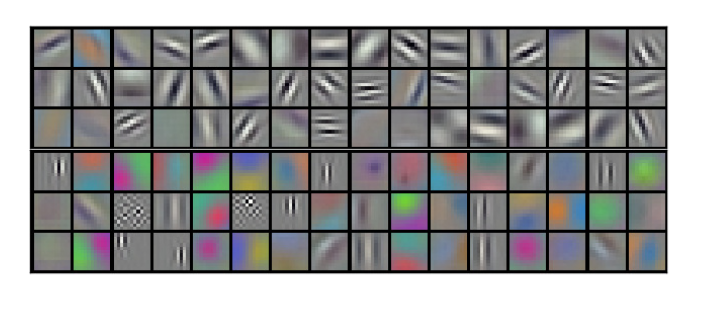
\includegraphics[width=0.75\textwidth]{img/fmap_imagenet}
            \caption{Kernels convolucionales de tamaño $11 \times 11 \times 3$ en la primera capa convolucional. Fuente: \cite{krizhevsky2012imagenet} }
            \label{fig:fmap_imagenet}
        \end{figure}
            
        Tal como se puede apreciar en la Figura(\ref{fig:fmap_imagenet}), en la primera capa convolucional, 
        los kernels de convolución corresponden con representaciones básicas en una imagen como la búsqueda de 
        bordes en distintas orientaciones, esto va acorde a lo establecido anteriormente en el modelo de 
        la corteza visual de un gato. Puede decirse entonces que las redes convolucionales emulan, en cierto modo, 
        al proceso biológico de visión en animales.

    \subsection{Sistemas de Aprendizaje Fin a Fin}

\section{Modelo cinemático del vehículo}
-
    \subsection{Ecuaciones de movimiento}


